%%%%%%%%%%%%%%%%%%%%%%%%%%%%%%%%%%%%%%%%%%%%%%%%%%%%%%%%%%%%%%%
%
% Welcome to writeLaTeX --- just edit your LaTeX on the left,
% and we'll compile it for you on the right. If you give
% someone the link to this page, they can edit at the same
% time. See the help menu above for more info. Enjoy!
%
%%%%%%%%%%%%%%%%%%%%%%%%%%%%%%%%%%%%%%%%%%%%%%%%%%%%%%%%%%%%%%%

% --------------------------------------------------------------
% This is all preamble stuff that you don't have to worry about.
% Head down to where it says "Start here"
% --------------------------------------------------------------
 
\documentclass[12pt]{article}
 
\usepackage[margin=1in]{geometry}
\usepackage{amsmath,amsthm,amssymb}

\usepackage{listings}
\usepackage{xcolor}

\usepackage{tikz}
\usetikzlibrary{shapes,positioning}

\tikzset{ell/.style={circle,draw,minimum height=0.5cm,minimum width=0.5cm,inner sep=0.2cm}}
\tikzset{rec/.style={rectangle,draw,minimum height=0.5cm,minimum width=0.5cm,inner sep=0.2cm}}

%New colors defined below
\definecolor{codegreen}{rgb}{0,0.6,0}
\definecolor{codegray}{rgb}{0.5,0.5,0.5}
\definecolor{codepurple}{rgb}{0.58,0,0.82}
\definecolor{backcolour}{rgb}{0.95,0.95,0.92}

%Code listing style named "mystyle"
\lstdefinestyle{mystyle}{
  backgroundcolor=\color{backcolour}, commentstyle=\color{codegreen},
  keywordstyle=\color{magenta},
  numberstyle=\tiny\color{codegray},
  stringstyle=\color{codepurple},
  basicstyle=\ttfamily\footnotesize,
  breakatwhitespace=false,         
  breaklines=true,                 
  captionpos=b,                    
  keepspaces=true,                 
  numbers=left,                    
  numbersep=5pt,                  
  showspaces=false,                
  showstringspaces=false,
  showtabs=false,                  
  tabsize=2
}

%"mystyle" code listing set
\lstset{style=mystyle}

 
\newcommand{\N}{\mathbb{N}}
\newcommand{\Z}{\mathbb{Z}}
 
\newenvironment{theorem}[2][Theorem]{\begin{trivlist}
\item[\hskip \labelsep {\bfseries #1}\hskip \labelsep {\bfseries #2.}]}{\end{trivlist}}
\newenvironment{lemma}[2][Lemma]{\begin{trivlist}
\item[\hskip \labelsep {\bfseries #1}\hskip \labelsep {\bfseries #2.}]}{\end{trivlist}}
\newenvironment{exercise}[2][Exercise]{\begin{trivlist}
\item[\hskip \labelsep {\bfseries #1}\hskip \labelsep {\bfseries #2.}]}{\end{trivlist}}
\newenvironment{problem}[2][Problem]{\begin{trivlist}
\item[\hskip \labelsep {\bfseries #1}\hskip \labelsep {\bfseries #2.}]}{\end{trivlist}}
\newenvironment{question}[2][Question]{\begin{trivlist}
\item[\hskip \labelsep {\bfseries #1}\hskip \labelsep {\bfseries #2.}]}{\end{trivlist}}
\newenvironment{corollary}[2][Corollary]{\begin{trivlist}
\item[\hskip \labelsep {\bfseries #1}\hskip \labelsep {\bfseries #2.}]}{\end{trivlist}}

\newenvironment{solution}{\begin{proof}[Solution]}{\end{proof}}
 
\begin{document}
 
% --------------------------------------------------------------
%                         Start here
% --------------------------------------------------------------
 
\title{Homework 7}%replace X with the appropriate number
\author{Mengxiang Jiang\\ %replace with your name
CSEN 5303 Foundations of Computer Science} %if necessary, replace with your course title
 
\maketitle

\begin{problem}{1}
    The \emph{intersection graph} of a collection of sets $A_1, A_2, \ldots, A_n$, is the graph that has a
vertex for each of these sets and has an edge connecting the vertices representing two sets if these
sets have a nonempty intersection.

Construct the intersection graph of these collections of sets.\\\\
1. Collection of sets $A_i, i=1..5$\\
$A_1 = \{0,2,4,6,8\}$\\
$A_2 = \{0,1,2,3,4\}$\\
$A_3 = \{1,3,5,7,9\}$\\
$A_4 = \{5,6,7,8,9\}$\\
$A_5 = \{0,1,8,9\}$
\begin{center}
    Intersection Table and Graph\\
    \begin{tabular}{|c|c|c|c|c|c|} 
     \hline
      & $A_1$ & $A_2$ & $A_3$ & $A_4$ & $A_5$\\
     \hline
     $A_1$ & - & \{0,2,4\} & $\emptyset$ & \{6,8\} & \{0,8\}\\ 
     $A_2$ & \{0,2,4\} & - & \{1,3\} & $\emptyset$ & \{0,1\}\\
     $A_3$ & $\emptyset$ & \{1,3\} & - & \{5,7\} & \{1,9\}\\
     $A_4$ & \{6,8\} & $\emptyset$ & \{5,7\} & - & \{8,9\} \\
     $A_5$ & \{0,8\} & \{0,1\} & \{1,9\} & \{8,9\} & - \\
     \hline
    \end{tabular}

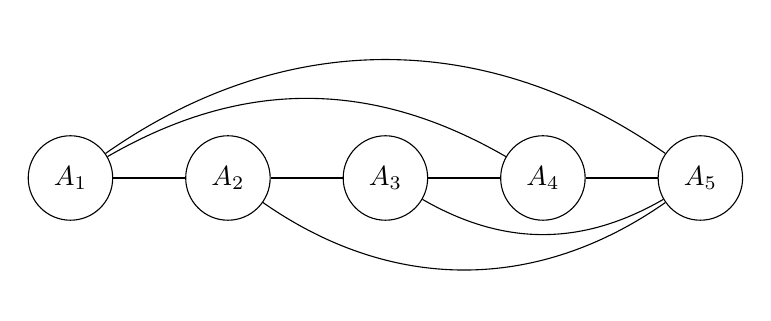
\begin{tikzpicture}[>=stealth]
    \node[ell] (a1)at (0,0) {$A_1$};
    \node[ell] (a2)at (2,0) {$A_2$};
    \node[ell] (a3)at (4,0) {$A_3$};
    \node[ell] (a4)at (6,0) {$A_4$};
    \node[ell] (a5)at (8,0) {$A_5$};

    \draw [] (a1) to []node[]{} (a2);
    \draw [] (a1) to [bend left]node[]{} (a4);
    \draw [] (a1) to [bend left=35]node[]{} (a5);
    \draw [] (a2) to []node[]{} (a3);
    \draw [] (a2) to [bend right=35]node[]{} (a5);
    \draw [] (a3) to []node[]{} (a4);
    \draw [] (a3) to [bend right]node[]{} (a5);
    \draw [] (a4) to []node[]{} (a5);
\end{tikzpicture}
\end{center}
\pagebreak
2. Collection of sets $A_i, i=1..5$\\
$A_1 = \{\ldots,-4,-3,-2,-1,0\}$\\
$A_2 = \{\ldots,-2,-1,0,1,2,\ldots\}$\\
$A_3 = \{\ldots,-6,-4,-2,0,2,4,6,\ldots\}$\\
$A_4 = \{\ldots,-5,-3,-1,1,3,5,\ldots\}$\\
$A_5 = \{\ldots,-6,-3,0,3,6,\ldots\}$
\begin{center}
    Intersection Table and Graph\\
    \begin{tabular}{|c|c|c|c|c|c|} 
     \hline
      & $A_1$ & $A_2$ & $A_3$ & $A_4$ & $A_5$\\
     \hline
     $A_1$ & - & $A_1$ & $\{\ldots, -2, 0\}$ & $\{\ldots, -3, -1\}$& $\{\ldots, -3, 0\}$\\ 
     $A_2$ & $A_1$ & - & $A_3$ & $A_4$ & $A_5$\\
     $A_3$ & $\{\ldots, -2, 0\}$ & $A_3$ & - & $\emptyset$ & $\{\ldots, -6, 0, 6, \ldots\}$\\
     $A_4$ & $\{\ldots, -3, -1\}$ & $A_4$ & $\emptyset$ & - & $\{\ldots, -9, -3, 3, 9, \ldots\}$ \\
     $A_5$ & $\{\ldots, -3, 0\}$ & $A_5$ & $\{\ldots, -6, 0, 6, \ldots\}$ & $\{\ldots, -9, -3, 3, 9, \ldots\}$ & - \\
     \hline
    \end{tabular}

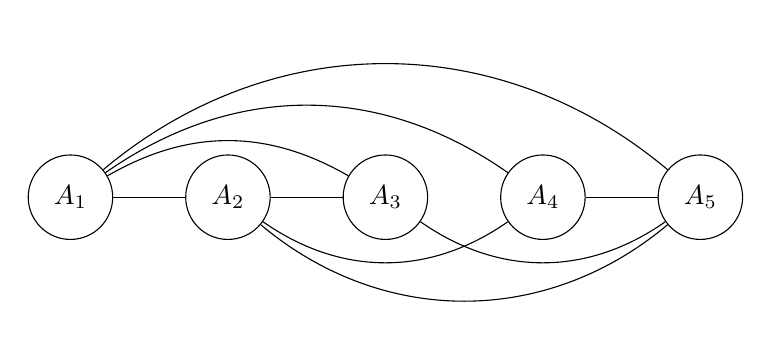
\begin{tikzpicture}[>=stealth]
    \node[ell] (a1)at (0,0) {$A_1$};
    \node[ell] (a2)at (2,0) {$A_2$};
    \node[ell] (a3)at (4,0) {$A_3$};
    \node[ell] (a4)at (6,0) {$A_4$};
    \node[ell] (a5)at (8,0) {$A_5$};

    \draw [] (a1) to []node[]{} (a2);
    \draw [] (a1) to [bend left]node[]{} (a3);
    \draw [] (a1) to [bend left=35]node[]{} (a4);
    \draw [] (a1) to [bend left=40]node[]{} (a5);
    \draw [] (a2) to []node[]{} (a3);
    \draw [] (a2) to [bend right=35]node[]{} (a4);
    \draw [] (a2) to [bend right=40]node[]{} (a5);
    \draw [] (a3) to [bend right=35]node[]{} (a5);
    \draw [] (a4) to []node[]{} (a5);
\end{tikzpicture}
\end{center} 
3. Collection of sets $A_i, i=1..5$\\
$A_1 = \{x|x<0\}$\\
$A_2 = \{x|-1<x<0\}$\\
$A_3 = \{x|0<x<1\}$\\
$A_4 = \{x|-1<x<1\}$\\
$A_5 = \{x|-1<x\}$\\
$A_6 = \mathbb{R}$
\begin{center}
    Intersection Table\\
    \begin{tabular}{|c|c|c|c|c|c|c|} 
     \hline
      & $A_1$ & $A_2$ & $A_3$ & $A_4$ & $A_5$ & $A_6$\\
     \hline
     $A_1$ & - & $A_2$ & $\emptyset$ & $A_2$& $A_2$ & $A_1$\\ 
     $A_2$ & $A_2$ & - & $\emptyset$ & $A_2$ & $A_2$ & $A_2$\\
     $A_3$ & $\emptyset$ & $\emptyset$ & - & $A_3$ & $A_3$ & $A_3$\\
     $A_4$ & $A_2$ & $A_2$ & $A_3$ & - & $A_4$ & $A_4$\\
     $A_5$ & $A_2$ & $A_2$ & $A_3$ & $A_4$ & - & $A_5$\\
     $A_6$ & $A_1$ & $A_2$ & $A_3$ & $A_4$ & $A_5$ & -\\
     \hline
    \end{tabular}
\pagebreak
\\Intersection Graph\\
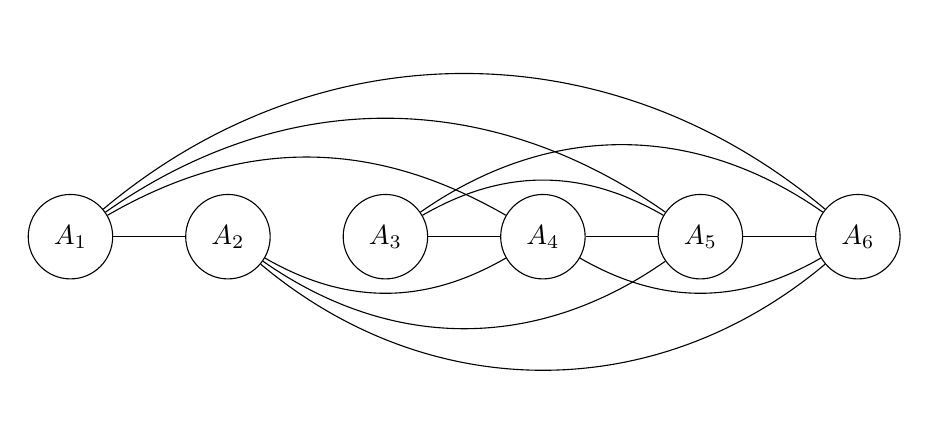
\begin{tikzpicture}[>=stealth]
    \node[ell] (a1)at (0,0) {$A_1$};
    \node[ell] (a2)at (2,0) {$A_2$};
    \node[ell] (a3)at (4,0) {$A_3$};
    \node[ell] (a4)at (6,0) {$A_4$};
    \node[ell] (a5)at (8,0) {$A_5$};
    \node[ell] (a6)at (10,0) {$A_6$};

    \draw [] (a1) to []node[]{} (a2);
    \draw [] (a1) to [bend left]node[]{} (a4);
    \draw [] (a1) to [bend left=35]node[]{} (a5);
    \draw [] (a1) to [bend left=40]node[]{} (a6);
    \draw [] (a2) to [bend right]node[]{} (a4);
    \draw [] (a2) to [bend right=35]node[]{} (a5);
    \draw [] (a2) to [bend right=40]node[]{} (a6);
    \draw [] (a3) to []node[]{} (a4);
    \draw [] (a3) to [bend left]node[]{} (a5);
    \draw [] (a3) to [bend left=35]node[]{} (a6);
    \draw [] (a4) to []node[]{} (a5);
    \draw [] (a4) to [bend right]node[]{} (a6);
    \draw [] (a5) to []node[]{} (a6);
\end{tikzpicture}
\end{center} 
\end{problem}

\begin{problem}{2}
    Consider the following program:\\
    $S_1:x:=0;$\\
    $S_2:x:=x+1;$\\
    $S_3:y:=2;$\\
    $S_4:z:=y;$\\
    $S_5:x:=x+2;$\\
    $S_6:y:=x+z;$\\
    $S_7:z:=4;$\\\\
    1. Show the different \emph{data dependencies} between all statements, including those that are not
    direct. Recall that there is a data dependency between two statements $S_i$ and $S_j$ if and only
    if $S_i$ computes the value of a variable that is used by $S_j$.\\\\
    $S_1:\emptyset$\\
    $S_2:\{S_1\}$\\
    $S_3:\emptyset$\\
    $S_4:\{S_3\}$\\
    $S_5:\{S_1, S_2\}$\\
    $S_6:\{S_1, S_2, S_3, S_4, S_5\}$\\
    $S_7:\emptyset$\\\\
    2. Construct the precedence graph for the above program. 

    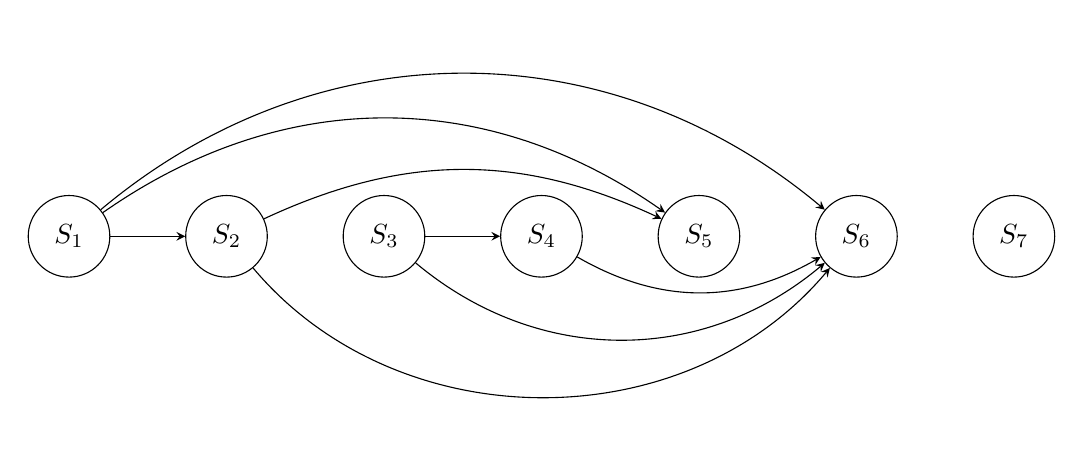
\begin{tikzpicture}[>=stealth]
        \node[ell] (s1)at (0,0) {$S_1$};
        \node[ell] (s2)at (2,0) {$S_2$};
        \node[ell] (s3)at (4,0) {$S_3$};
        \node[ell] (s4)at (6,0) {$S_4$};
        \node[ell] (s5)at (8,0) {$S_5$};
        \node[ell] (s6)at (10,0) {$S_6$};
        \node[ell] (s7)at (12,0) {$S_7$};
    
        \draw [->] (s1) to []node[]{} (s2);
        \draw [->] (s1) to [bend left=35]node[]{} (s5);
        \draw [->] (s1) to [bend left=40]node[]{} (s6);
        \draw [->] (s2) to [bend left=25]node[]{} (s5);
        \draw [->] (s2) to [bend right=50]node[]{} (s6);
        \draw [->] (s3) to []node[]{} (s4);
        \draw [->] (s3) to [bend right=40]node[]{} (s6);
        \draw [->] (s4) to [bend right]node[]{} (s6);
    \end{tikzpicture}
\end{problem}
\pagebreak
\begin{problem}{3}
    Suppose that a new company has five employees: Zamora, Agraharam, Smith, Chou,
    and Macintyre. Each employee will assume one of six responsibilities, namely planning, publicity,
    sales, marketing, development, and industry relations. Each employee is capable of doing one or
    more of these jobs. Zamora could do planning, sales, marketing, or industry relations. Agraharam
    could do planning or development. Smith could do publicity, sales, or industry relations. Chou
    could do planning, sales, or industry relations. Macintyre could do planning, publicity, sales, or
    industry relations.\\\\
    1. Model the capabilities of these employees using a bipartite graph.\\\\
    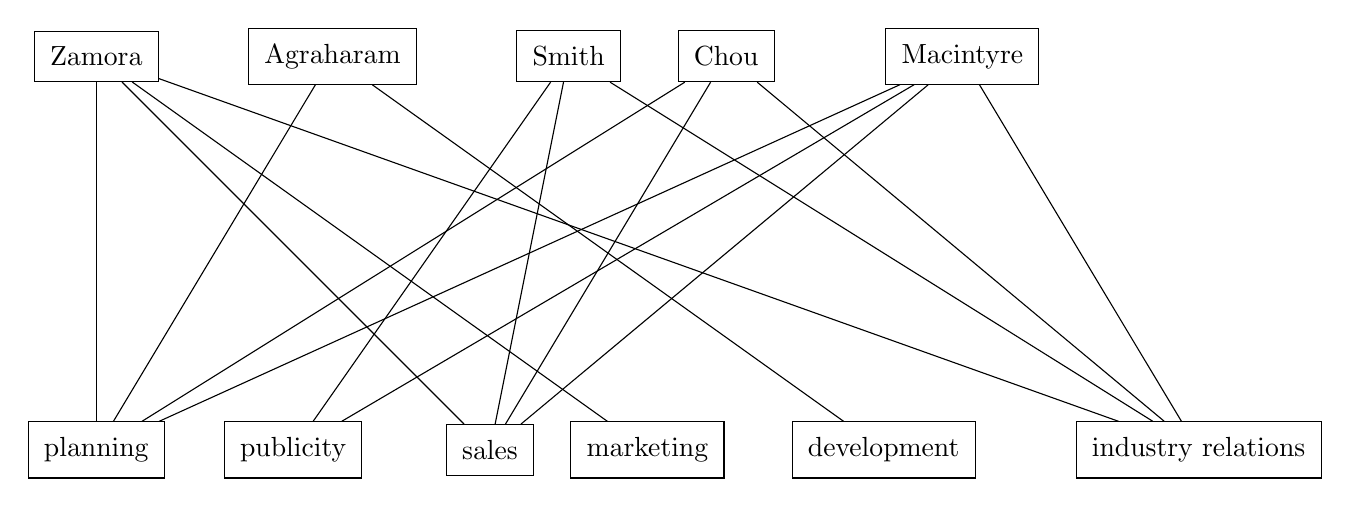
\begin{tikzpicture}[>=stealth]
        \node[rec] (z)at (0,5) {Zamora};
        \node[rec] (a)at (3,5) {Agraharam};
        \node[rec] (s)at (6,5) {Smith};
        \node[rec] (c)at (8,5) {Chou};
        \node[rec] (m)at (11,5) {Macintyre};

        \node[rec] (r1)at (0,0) {planning};
        \node[rec] (r2)at (2.5,0) {publicity};
        \node[rec] (r3)at (5,0) {sales};
        \node[rec] (r4)at (7,0) {marketing};
        \node[rec] (r5)at (10,0) {development};
        \node[rec] (r6)at (14,0) {industry relations};
    
        \draw [] (z) to []node[]{} (r1);
        \draw [] (z) to []node[]{} (r3);
        \draw [] (z) to []node[]{} (r4);
        \draw [] (z) to []node[]{} (r6);

        \draw [] (a) to []node[]{} (r1);
        \draw [] (a) to []node[]{} (r5);

        \draw [] (s) to []node[]{} (r2);
        \draw [] (s) to []node[]{} (r3);
        \draw [] (s) to []node[]{} (r6);

        \draw [] (c) to []node[]{} (r1);
        \draw [] (c) to []node[]{} (r3);
        \draw [] (c) to []node[]{} (r6);

        \draw [] (m) to []node[]{} (r1);
        \draw [] (m) to []node[]{} (r2);
        \draw [] (m) to []node[]{} (r3);
        \draw [] (m) to []node[]{} (r6);
    \end{tikzpicture}
    2. Find an assignment of responsibilities such that each employee is assigned a responsibility.\\
    Since only Zamora can do marketing, he is assigned marketing.\\
    Likewise, Agraharam is assigned development.\\
    Let Smith handle publicity.\\
    Let Chou handle planning.\\
    Macintyre can then handle sales.\\

\end{problem}
% --------------------------------------------------------------
%     You don't have to mess with anything below this line.
% --------------------------------------------------------------
 
\end{document}